
\documentclass{article}
\usepackage{mathrsfs}
\usepackage{mathtools}
\usepackage{bm}
\usepackage{bbm}
\usepackage{amsmath,amsfonts,amssymb,amsthm,rotating}
\usepackage{xcolor}
\usepackage{hyperref}
\usepackage{enumerate}
\usepackage[authoryear,longnamesfirst,round]{natbib}
\usepackage[left = 2.5cm, right = 2.5cm, top = 3cm, bottom = 2.5cm]{geometry}
\usepackage{setspace}
\usepackage[nottoc]{tocbibind}

% custom enviroments
\newtheorem{defn}{Definition}
\newtheorem{prop}{Proposition}
\newtheorem{lemma}{Lemma}
\newtheorem{thm}{Theorem}
\newtheorem{cor}{Corollary}
\newtheorem*{exmpl}{Running example}



\begin{document}
\title{%
  \textbf{ \huge The Hilbert Projection Theorem \\
  \large Some Applications in Statistical Estimation and Time Series Forecasting}}

\author{\textbf{Laura Ventosa Andreu (EME09)} \\
Prof. Christian Brownlees \\
Universitat Pompeu Fabra}
\date{Academic Year 2018-2019}
\maketitle


\begin{abstract}
This thesis focuses on the Projection Theorem in the context of Hilbert spaces and how it can be extended to the field of statistical estimation and time series forecasting. The projection theorem is a mathematical result which guarantees that, under some conditions, an element (i.e. a point) belonging to a Hilbert space can be projected onto a closed subspace or a closed and convex subset in a way that the distance between the element and the surface onto which it is projected is minimized. Depending on the surface where the element is projected, the projection will present some peculiarities, which will be studied in detail. In the world of statistics and forecasting, this theorem allows us to state that the minimum variance estimator for the parameters of a regression model will exist and be unique if some conditions are satisfied. Finally, the paper also deals with the connection between the conditional expectation and the best linear prediction using the result and implications of the projection theorem. \newline
\end{abstract}

\textit{Keywords}: Projection theorem, orthogonal projection, projection onto a convex set, best linear prediction

\newpage

\tableofcontents

\newpage

\section{Introduction} 
In a world filled with uncertainty, there is little we can do to ensure that the actions and events that revolve around us happen the way we want to or are consistent with the way we expect them to be. In our daily lives, we all try to minimize such uncertainty: from checking the weather before choosing what to wear to making a prediction about how much food and drinks will be needed when throwing a party at our house. But, what is forecasting and why is it important? \newline

Despite not having a unified and clear definition of what forecasting really means, one can say that the term refers to the process of using information about the past and even the present to build or obtain some information about the future. In particular, statistical forecasting is a field of study which predicts future values of a given variable using its past and present values and analyzing trends and patterns with the objective of decreasing the level of uncertainty and risk. Forecasting, especially in the field of economics, finance and business, is important because it allows us to adapt better to imminent economic scenarios, either good or bad, as well as to reduce the risk and uncertainty inherent to these fields. Forecasts present different degrees of accuracy, which depend on the amount and quality of data and the model or specification used, among other factors. Likewise, there is a trade-off between the fit of the model and its forecasting ability, in the sense that models which fit the data very well may have a poor forecasting performance. In general, however, highly accurate forecasting is not that necessary. \newline

Nevertheless, one cannot undermine the widespread opinion that economic and financial forecasts are often wrong. Forecasts can fail at predicting the near future due to modeling errors, bad quality data or even bad luck. To decrease the probability of having inaccurate or even wrong forecasts, statisticians usually work with an optimal forecast. An optimal forecast is obtained by minimizing the conditional expectation of a chosen loss function. \newline

In this thesis we will be working with Hilbert spaces, which allow us to use the same vector algebra and calculus notions used in two-dimensional Euclidean planes and three-dimensional spaces but with the possibility of working in any finite or infinite number of dimensions. Mathematical concepts, in particular those involving a lot of abstraction and infinite dimensions, may be seen as anything but natural and very disconnected from reality. Nonetheless, the Hilbert projection theorem and its implications are very much used in statistical estimation and forecasting since, among other things, they are a way of easing our computations. \newline

The paper is organized as follows: the first section reviews and defines some key mathematical concepts to be able to understand more complex mathematical notions presented later in the paper. The second section is about the projection theorem, the key result of this thesis, which is studied under three scenarios: a point projected onto a closed subspace, a projection onto a set that is closed and convex and projections involving heterogeneous variables. In order to assist a better understanding and visualization on how the different projections would look like, some self-made diagrams are attached. Moreover, in that same section, autoregressive processes for time series data are introduced and we prove that the projection theorem and its implications can be extended to this kind of specification as well. Lastly, in the third section, we talk about the best linear prediction in a probability space and its relation to the conditional expectation of a random variable given another random variable.

\newpage

\section{Preliminaries on Hilbert Spaces}
In this section we are going to, first, define some mathematical concepts and definitions relevant for the topic of this project and, second, set the basic framework for Hilbert spaces. The definitions and mathematical notions in this section and the following one have been extracted from chapter 2 of \citet{BrockwellDavis:1991} and the same notation is used. \newline

\begin{defn}[Vector space]
A \textbf{vector space $V$} is a set that is closed under finite vector addition and scalar multiplication. A vector space must satisfy commutativity, associativity of vector addition, associativity of scalar multiplication, distributivity of scalar sums, distributivity of vector sums, the additive identity, the negative identity and the scalar multiplication identity.
\end{defn}

One example of vector space is the $n$-dimensional Euclidean space $\mathbb{R}^n$, where each element is represented by a list of $n$ real numbers. \newline

\begin{defn}[Inner-product space]
An \textbf{inner-product space} is a generalization of the dot product or scalar product of two vectors in an $n$-dimensional Euclidean space. In other words, an inner product space is a vector space where each pair of vectors is associated with a scalar quantity known as inner product of those two vectors. The inner product is denoted as $\langle \cdot , \cdot \rangle$.  \newline
\end{defn}

\begin{defn}[Norm]
The \textbf{norm} of an element $x$ of an inner-product space is, by definition, 
\[
\lVert {x} \rVert = \sqrt{\langle x,x \rangle}.
\]
\end{defn}

In the Euclidean space $\mathbb{R}^n$, the norm of a vector is simply its length. It may also be useful to introduce the \textbf{Cauchy-Schwarz inequality}: 
\[
\left|\langle x,y \rangle\right| \leqslant \lVert {x} \rVert \lVert {y} \rVert.
\]

Another important inequality is the \textbf{Triangle inequality}, expressed as
\[
\lVert x + y \rVert \leqslant \lVert {x} \rVert + \lVert {y} \rVert.
\]

\begin{defn}[Convergence in norm]
A sequence $\{x_n\}$ \textbf{converges in norm} if, as  $n$ $\rightarrow$ $\infty$, 
\[
\lVert x_n - x \rVert \rightarrow 0, 
\] where $x$ is known as the limit of the sequence. \newline
\end{defn}

\begin{defn}[Cauchy sequence]
A sequence is said to be \textbf{Cauchy} if its elements come arbitrarily close to each other as $n,m \rightarrow \infty$. Equivalently,
\[
\lVert x_n - x_m \rVert \rightarrow 0 
\]
\end{defn}

Moreover, if every Cauchy sequence in a space is convergent (i.e. the sequence approaches its limit as it progresses) that space is \textbf{complete}. \newline

\begin{defn}[Hilbert space]
A \textbf{Hilbert space}, denoted as $\mathscr{H}$,  is a generalisation of the notion of Euclidean space. In other words, a Hilbert space is an extension of vector algebra and calculus to spaces of any finite and infinite number of dimensions. Moreover, a Hilbert space is an inner-product space with the additional property of completeness (i.e. every Cauchy sequence $\{x_n\}$ converges in norm to some element x $\in$ $\mathscr{H}$). 
\end{defn}

In addition, the inner-product of a Hilbert space corresponds to $\langle X, Y \rangle = \mathbb E(XY)$. With notions of basic statistics, it can be observed that this inner-product definition corresponds to a covariance. This inner-product implies that an estimator $\hat{X}$ that minimizes the norm of the estimation error $\lVert X - \hat{X}\rVert$, understood as the difference between the observed value of $X$ and the best linear predictor in this case, also minimizes the variance since $\lVert X - \hat{X}\rVert$ = $\sqrt{\mathbb E(X - \hat{X})(X - \hat{X})'}$. \newline

\begin{exmpl}
The set of all real numbers $\mathbb{R}$ is a Hilbert space as it is an inner-product space that is complete since it can be proved that in $\mathbb{R}$ a sequence is Cauchy if and only if it is convergent. \newline
\end{exmpl}

\begin{defn}[Linear subspace]
A \textbf{linear subspace} is a vector space that is contained within another vector space. \newline
\end{defn}

\begin{defn}[Closed subspace]
A linear subspace $\mathscr{M}$ of a Hilbert space $\mathscr{H}$ is said to be a \textbf{closed subspace} of $\mathscr{H}$ if it contains all of its limit points (i.e. if $\{x_n\}$ $\in$ $\mathscr{M}$ and $\lVert x_n - x \rVert$ $\rightarrow$ 0 imply that x $\in$ $\mathscr{M}$).  
\end{defn}
Moreover, a linear subspace of a Hilbert space is a Hilbert space itself. \newline

\begin{prop}[Continuity of the inner-product]\label{prop:cip}
 If $\{x_n\}$ and $\{y_n\}$ are sequences of elements of the inner-product space $\mathscr{H}$ such that $\lVert x_n - x \rVert$ $\rightarrow$ 0 and $\lVert y_n - y \rVert$ $\rightarrow$ 0, then 
 \begin{enumerate}
   \item $\lVert x_n \rVert$ $\rightarrow$ $\lVert x \rVert$
   \item $\langle x_n, y_n \rangle$ $\rightarrow$ $\langle x,y \rangle$ 
\end{enumerate}
\end{prop}

\begin{proof}[Proof of Proposition \ref{prop:cip}]
From the triangle inequality it follows that $\lVert x \rVert$ $\leqslant$ $\Vert x - y \rVert$ + $\lVert y \rVert$ and $\lVert y \rVert$ $\leqslant$ $\lVert y - x \rVert$ + $\lVert x \rVert$. From these two statements we get that: $\lVert y - x \rVert$ $\geqslant$ $\left| \lVert  x  \rVert \lVert  y  \rVert \right|$, from which the first part of the proposition follows immediately. Moreover, by the Cauchy-Schwarz inequality
\[
\left|\langle x_n, y_n \rangle - \langle x, y \rangle \right| = \left|\langle x_n, y_n - y \rangle + \langle x_n - x, y \rangle \right| \leqslant \left|\langle x_n, y_n - y \rangle\right|+ \left|\langle x_n - x, y \rangle \right| \leqslant \lVert x_n \rVert \lVert y_n - y\rVert + \lVert x_n - x \rVert \lVert y \rVert.
\] 
Further, because $\lVert x_n \rVert$ $\rightarrow$ $\lVert x \rVert$, we can conclude that $\left|\langle x_n, y_n \rangle - \langle x,y \rangle\right|$ $\rightarrow$ 0 as n $\rightarrow$ $\infty$. \newline
\end{proof}

The \textbf{Parallelogram Law} will also be useful in the next section. This result states that, if $\mathscr{H}$ is an inner-product space, then
\[
\lVert x + y\rVert^2 + \lVert x - y\rVert^2 = \lVert x \rVert^2 + \lVert y\rVert^2.
\]

\begin{defn}[Orthogonality]
Two vectors $x$ and $y$ are \textbf{orthogonal} or \textbf{perpendicular} if their scalar or inner-product is 0. Orthogonality is denoted as $x \bot y$. 
\end{defn}

In this thesis, we will rather focus on the \textbf{orthogonal complement} of $\mathscr{M}$, denoted by $\mathscr{M^\bot}$, which contains all the elements of  $\mathscr{H}$ orthogonal to every element of $\mathscr{M}$. Thus, $x$ $\in$ $\mathscr{M^\bot}$ if and only if $\langle x,y \rangle = 0$ for all $y$ $\in$ $\mathscr{M}$. \newline

\begin{prop}\label{prop:coc}
If $\mathscr{M}$ is any subspace of a Hilbert space $\mathscr{H}$ then $\mathscr{M^\bot}$ is a closed subspace of $\mathscr{H}$.
\end{prop}

\begin{proof}[Proof of proposition \ref{prop:coc}]
From the previous definition, 0 $\in$ $\mathscr{M^\bot}$. If $x_1, x_2$ $\in$ $\mathscr{M^\bot}$ then all linear combinations of ${x_1}$ and ${x_2}$ will belong to $\mathscr{M^\bot}$. Thus, $\mathscr{M^\bot}$  is a subspace of $\mathscr{H}$. If $x_n$ $\in$ $\mathscr{M^\bot}$ and $\lVert x_n - x \rVert$ $\rightarrow$ 0, then by previous results $\langle x,y \rangle$ = 0 for all y $\in$ $\mathscr{M}$, so $x$ $\in$ $\mathscr{M^\bot}$ and, therefore, $\mathscr{M^\bot}$ is closed. \newline
\end{proof}

As mentioned earlier, Hilbert spaces can be related to random variables. Let $(\Omega, \mathscr{F}, P)$ be a probability space and $C$ be the collection of all random variables X defined on $\Omega$ such that 
\[ \mathbb EX^2 = \int_\Omega X(\omega )^2P(d\omega) < \infty.\] 

As we have that for all a $\in$ $\mathbb{R}$ and X $\in$ $C$ \[ \mathbb E(aX)^2 = a^2 \mathbb EX^2 < \infty,\]
then $C$ is a vector space. The collection $C$ of random variables satisfying the above condition can also be denoted as $L^2$ and this is the notation that will be used from now on in the paper. $\Omega$ is the set of all possible outcomes, $\mathscr{F}$ refers to the $\sigma$-algebra representing the collection of all events and $P$ corresponds to the probabilities of such events. \newline

In particular, $L^2(\Omega, \mathscr{F}, P)$ is a Hilbert space with the inner product being $\langle X, Y \rangle = \mathbb E(XY)$, where $X$ and $Y$ are two arbitrary random variables belonging to $L^2$. To show that $L^2$ is a Hilbert space it suffices to show completeness. In other words, we need to show that if $X_n$ belongs to $L^2$ and $\lVert X_n - X_m \rVert$ $\rightarrow$ 0 as $m, n \rightarrow 0$, then there exists a vector $X \in L^2$ such that $X_n \rightarrow X$ in mean square, where $X$ is the limit of a converging subsequence of ${X_n}$, meaning that the squared difference between both elements tends to 0. Before introducing the proof of completeness of $L^2$, we need the following proposition.\newline

\begin{prop} \label{prop:lc}
If $X_n \in L^2$ and $\lVert X_{n+1} - X_n \rVert \leqslant 2^{-k}$ there there exists a random variable X belonging to $(\Omega, \mathscr{F}, P)$ such that $X_n \rightarrow X$ with probability 1.
\end{prop}

\begin{proof}[Proof of Proposition \ref{prop:lc}]
Let $X_0 = 0$, then $X_n = \sum_{j=1}^{n}(X_j - X_{j-1})$. By the monotone convergence theorem \footnote{The \textbf {monothone convergence theorem} states that an increasing sequence that is bounded above by a supremum will converge to such supremum and that a decreasing sequence that is bounded below by an infimum will converge to such infimum} and the Cauchy-Schwarz inequality,
\[
\mathbb E \sum_{j=1}^{\infty} \lVert X_j - X_{j-1}\rVert = \sum_{j=1}^{\infty} \mathbb E \left| X_j - X_{j-1}\right| \leqslant \sum_{j=1}^{\infty} \lVert X_j - X_{j-1} \rVert \leqslant \lVert X_1 \rVert + \sum_{j=1}^{\infty} 2^{-j} < \infty
\]

Therefore, $\lim_{n\to\infty} \sum_{j=1}^{\infty} \lVert X_j - X_{j-1} \rVert$ and $\lim_{n\to\infty} \sum_{j=1}^{\infty} (X_j - X_{j-1})$ exist and are finite with probability one. \newline
\end{proof}


\begin{lemma}[Fatou's Lemma]
If ${f_n}$ is a sequence of non-negative measurable functions, then 
\[
\int \lim_{n\to\infty} \inf f_n d\mu = \lim_{n\to\infty} \inf \int f_n d\mu. 
\]
\end{lemma}
We are going to take this lemma as given and not going to prove it as iits proof involves measure theory. \newline

\begin{thm}[Completeness of $L^2$]\label{thm:l2c}
$L^2(\Omega, \mathscr{F}, P)$ is complete.
\end{thm}

\begin{proof}[Proof of Theorem \ref{thm:l2c}]
If ${X_n}$ is a Cauchy sequence in $L^2$ then we can find integers $n_1<n_2<...$ and also $\lVert X_n - X_m \rVert \leqslant 2^{-k}$ for $n, m > n_k$. We need to choose $n_1, n_2, ...$ so that Proposition 3 is satisfied for $k=1$.
By such proposition, we know that there exists a random variable $X$ such that $X_{n_k}$ $\rightarrow$ $X$ with probability 1 as $k\rightarrow \infty$. 
\[
\lVert X_n - X_m \rVert^2 = \int \left| X_n - X_m \right|^2 dP = \int \lim_{k\to\infty} \inf \left| X_n - X_{n_k} \right|^2 dP.
\]
Using the above lemma as well, we get $\lVert X_n - X \rVert^2$ $\leqslant$ $\lim_{k\to\infty} \inf \lVert X_n - X_{n_k} \rVert^2$.
As ${X_n}$ is a Cauchy sequence, with $n$ large enough, the right hand side of this last expression can be made arbitrarily small and, thus, $\lVert X_n - X\rVert^2$ $\rightarrow$ 0.
Moreover, from the triangle inequality: $\lVert X \rVert$ $\leqslant$  $\lVert X_n - X \rVert$ + $\lVert X_n \rVert$, which has a finite right-hand side for a large enough $n$. Hence, $L^2$ is a vector space that is complete as well, making it a Hilbert space. \newline
\end{proof}

\begin{prop}[Norm convergence]\label{prop:nc}
 If $\{x_n\}$ is a sequence of elements belonging to a Hilbert space $\mathscr{H}$, then $\{x_n\}$ converges in norm if and only if 
\[
\lVert x_n - x_m \rVert \rightarrow 0,\] as m, n $\rightarrow$ $\infty$.
\end{prop}
 
\begin{proof}[Proof of Proposition \ref{prop:nc}]
The proof follows from the fact that as we are referring to a Hilbert space, $\mathscr{H}$ is complete and, thus, every Cauchy sequence is norm-convergent in $\mathscr{H}$ by definition. Moreover, by the triangle inequality:
\[
\lVert {x_n - x_m} \rVert \leqslant \lVert {x_n - x} \rVert + \lVert {x - x_m} \rVert.
\]
\end{proof}

\begin{defn}[Mean-squared convergence]
Norm convergence of $\{X_n\}$ to X in an $L^2$ space is known as \textbf{mean-squared convergence}. \newline
\end{defn}

\begin{defn}[Projection]
Let $S$ be an arbitrary subset of a larger set. The vector $x_p$ is a $\textbf{projection}$ of $x$ on $S$ if $x_p$ $\in$ $S$ and $\lVert x - x_p\rVert$ $\leqslant$ $\lVert x - s\rVert$ for all $s$ $\in$ $S$.
\end{defn}
Closeness of a subset or a subspace is a necessary condition for the projection to exist. However, it is not a sufficient condition. The subset or subspace in question will have to be complete as well in order for us to be able to claim that the projection will, for sure, exist. Nonetheless, as we are working with Hilbert spaces $\mathscr{H}$, which are complete by definition, any of the subsets or subspaces of $\mathscr{H}$ will be complete as well. Thus in this thesis, closeness is a necessary and sufficient condition for the existence of a given projection.

\newpage

\section{Projection Theorem in the Context of Hilbert Spaces}

After introducing some relevant and necessary mathematical concepts in the previous section, we will now finally focus on the main notion of this project: the \textbf{Projection Theorem}. And, as we evaluate the theorem in question in the context of Hilbert spaces, we may as well call it the Hilbert Projection Theorem.

\subsection{Projection onto a Closed Subspace}

\begin{thm}[Projection Theorem]\label{thm:prj}
Let $\mathscr{M}$ be a closed subspace of the Hilbert space $\mathscr{H}$ and $x$ $\in$ $\mathscr{H}$, then: 
\begin{enumerate}[(i)]
   \item There exists a unique element $\hat{x}$ $\in$ $\mathscr{M}$ such that $\lVert x - \hat{x}\rVert$ = $\inf_{y \in \mathscr{M}} \lVert x - y \rVert$, and
   \item $\hat{x}$ $\in$ $\mathscr{M}$ and $\lVert x - \hat{x}\rVert$ = $\inf_{y \in \mathscr{M}} \lVert x - y \rVert$ if and only if $\hat{x}$ $\in$ $\mathscr{M}$ and (x - $\hat{x}$) $\in$ $\mathscr{M^\bot}$. 
\end{enumerate}
In particular, the element $\hat{x}$ is called the (orthogonal) projection of x onto $\mathscr{M}$.
\end{thm}

\begin{proof}[Proof of Theorem \ref{thm:prj}] 
$(i)$ If $d$ = $\inf_{y \in \mathscr{M}} \lVert x - y \rVert^2$ then there is a sequence ${y_n}$ of elements of $\mathscr{M}$ such that $\lVert y_n - x \rVert^2$ $\rightarrow$ $d$. By applying the parallelogram law and using the fact that $(y_m + y_n)/2$ $\in$ $\mathscr{M}$, we have that:
\[ 
0 \leqslant \lVert y_m - y_n \rVert^2 = -4\lVert (y_m + y_n)/2 - x \rVert^2 + 2(\lVert y_n - x \rVert^2 + \lVert y_m - x \rVert^2) \leqslant -4d + 2(\lVert y_n - x \rVert^2 + \lVert y_m - x \rVert^2) \rightarrow 0,
\]
as $n, m \rightarrow \infty$.
Hence, by the Cauchy criterion, we know that there exists a $\hat{x}$ $\in$ $\mathscr{M}$ such that $\lVert y_n - \hat{x}\rVert \rightarrow 0$. Furthermore, as $\hat{x} \in \mathscr{M}$ and applying the continuity of the inner-product, 
\[ 
\lVert x - \hat{x}\rVert^2 = \lim_{n\to\infty} \lVert x - y_n\rVert^2 = d.
\]
However, we should also check for uniqueness. To do so, suppose that $\hat{y}$ $\in$ $\mathscr{M}$ as well as 
\[
\lVert x - \hat{y}\rVert^2 = \lVert x - \hat{x}\rVert^2 = d,
\]
and apply, again, the parallelogram law: 
\[
0 \leqslant \lVert \hat{x} - \hat{y} \rVert^2 = -4\lVert (\hat{x} +\hat{y})/2 - x \rVert^2 + 2(\lVert \hat{x} - x \rVert^2 + \lVert \hat{y} - x \rVert^2) \leqslant -4d + 4d = 0.
\]
Thus, $\hat{y}$ = $\hat{x}$ and this proves uniqueness. \newline

$(ii)$ If $\hat{x}$ $\in$ $\mathscr{M}$ and (x - $\hat{x}$) $\in$ $\mathscr{M^\bot}$ then $\hat{x}$ is the unique element of $\mathscr{M}$ defined in the first part of this theorem as for any y $\in$ $\mathscr{M}$ 
\[ 
\lVert x - y \rVert^2 = \langle x - \hat{x} + \hat{x} - y, x - \hat{x} + \hat{x} - y\rangle = \lVert x - \hat{x}\rVert^2 + \lVert \hat{x} - y \rVert^2 \geqslant \lVert x - \hat{x}\rVert^2,
\]
with equal sign if and only if $\hat{x}$ = y. 
Conversely, if $\hat{x}$ $\in$ $\mathscr{M}$ and (x - $\hat{x}$) $\notin$ $\mathscr{M^\bot}$ then $\hat{x}$ is not the element of $\mathscr{M}$ closest to x as $\overline{x}$ = $\hat{x}$ + $ay/\lVert y \rVert^2$ is closer to $x$, where y is any element belonging to $\mathscr{M}$ satisfying $\langle x - \hat{x},y \rangle$ $\neq$ 0 and $a=\langle x - \hat{x},y \rangle$.
\end{proof}

Given a Hilbert space $\mathscr{H}$, a closed subspace $\mathscr{M}$ and an element x $\in$ $\mathscr{H}$, the projection theorem shows that the element of $\mathscr{M}$ closest to x exists and is the unique element $\hat{x}$ $\in$ $\mathscr{M}$ such that $\langle x - \hat{x},y \rangle$ = 0 for all $y \in \mathscr{M}$. \newline

The projection theorem ensures that an estimator, the errors of which are orthogonal, is the (linear) minimum variance estimator. Hence, this theorem can be used to find the minimum variance estimate of a vector of random variables with finite variances as a function of some other finite variance random variables. This statement can help us understand why Ordinary Least Squares (OLS from now on) estimation, which is deeply entangled with the projection theorem and provides estimates with the minimum variance, is very much used. In particular, OLS estimation can be interpreted as a projection onto the linear space spanned by the independent variables that act as regressors. The following scenarios are practical examples of the projection theorem in particular Hilbert spaces. \newline

\begin{exmpl}
Imagine we are in $\mathbb{R}^3$ and the values of the vectors $y$, $x_1$ and $x_2$, where y is a linear combination of $x_1$ and $x_2$, are known. Further, the coefficients of $x_1$ and $x_2$ are not known. The best linear approximation will be $\hat{y} = \alpha_1x_1 + \alpha_2x_2$ such that the distance between $\hat{y}$ and the real value of $y$ is minimized. In other words, S = $\lVert y -  \alpha_1x_1 - \alpha_2x_2 \rVert^2$ is minimum.
There are two ways of solving this problem:
\begin{enumerate}
\item We can use calculus to obtain the partial derivatives of S with respect to $x_1$ and $x_2$, make them equal to 0 and solve for $\alpha_1$ and $\alpha_2$. These two values will be the estimates of the coefficients in the linear combination y that minimize S.
\item We can take a the geometric approach and observe that the vector $\hat{y}$ is the vector in the plane determined by $x_1$ and $x_2$ such that $y - \alpha_1x_1 + \alpha_2x_2$ is orthogonal to the 2-dimensional plane spanned by $x_1$ and $x_2$. Hence, the orthogonality condition can be expressed as: $\langle y - \alpha_1x_1 - \alpha_2x_2, x_i \rangle$ = 0 for $i = 1,2...$ \newline
\end{enumerate} 
\end{exmpl}

The following diagram may help visualize the geometric approach to an orthogonal projection, where a point $x$ is projected onto a closed subspace $A$ and $\hat{x}$ is the orthogonal projection of $x$.

\begin{center}
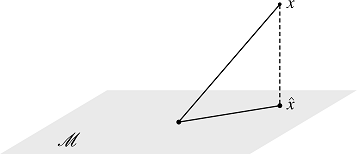
\includegraphics{fig1.png} \newline
\end{center}

\begin{exmpl}
The case of the linear approximation in $L^2(\Omega, \mathscr{F}, P)$ is also interesting. Let ${X_1}$, ${X_2}$ and $Y$ be random variables in the space $L^2(\Omega, \mathscr{F}, P)$. If only ${X_1}$ and ${X_2}$ are observed we will have to estimate the value of $Y$ by using the linear combination $\hat{Y} = \alpha_1X_1 + \alpha_2X_2$, which is analogous to the one in the previous example. Further, $\hat{Y}$ minimizes the mean squared error defined as \[S = \mathbb E|Y - \alpha_1X_1 - \alpha_2X_2|^2 = \lVert Y -  \alpha_1X_1 - \alpha_2X_2 \rVert^2.\]
The logic behind this problem is the same logic used by the OLS method used in statistics and econometrics, where the difference between the observed and the estimated value of $Y$ given the values for $X_1$ and $X_2$ is defined as the residual. As in the example above, there are two ways of solving this problem: using calculus or the alternative geometric approach. If we choose the latter, we will want to find an element $\hat{Y}$ in the following set: 
\[
\mathscr{M} = \{X \in L^2(\Omega, \mathscr{F}, P) : X = a_1X_1 + a_2X_2
\] 
for some $a_1, a_2 \in \mathbb{R}$ such that $\lVert Y -  \hat{Y} \rVert^2$ is minimized. By the projection theorem and analogously to the previous example, $\hat{Y}$ will satisfy the condition establishing that the vector $Y - \hat{Y}$ is orthogonal to all the elements in $\mathscr{M}$. The orthogonality condition now becomes $\langle Y - \alpha_1X_1 - \alpha_2X_2, X \rangle$ = 0. By linearity of the inner-product, this expression can be rewritten as $\langle Y - \alpha_1X_1 - \alpha_2X_2, X_i \rangle$ = 0 for $i = 1,2$, which can be, at the same time, written as
\[
\alpha_1 \mathbb E(X_1^2) + \alpha_2 \mathbb E(X_1X_2) = \mathbb E(YX_1),
\]
\[
\alpha_1 \mathbb E(X_1X_2) + \alpha_2 \mathbb E(X_2^2) = \mathbb E(YX_2).
\]
\end{exmpl}

Following this last example, it must be highlighted that if $Y$, $X_1$ and $X_2$ are in a well defined space we do not need to minimize the variance directly when estimating the parameters of interest $\alpha_1$ and $\alpha_2$ since the projection theorem ensures that a prediction with orthogonal errors is the (linear) minimum variance estimate. This is treated in more detail in section 4.\newline

\begin{cor}[Projection Mapping of $\mathscr{H}$ onto $\mathscr{M}$]
If $\mathscr{M}$ is a closed subspace of the Hilbert space $\mathscr{H}$ and $I$ is the identity mapping on $\mathscr{H}$, then there exists a unique mapping $P_\mathscr{M}$ of $\mathscr{H}$ onto $\mathscr{M}$ such that $I - P_\mathscr{M}$ maps $\mathscr{H}$ onto $\mathscr{M^\bot}$. $P_\mathscr{M}$ is called the projection mapping of $\mathscr{H}$ onto $\mathscr{M}$. Moreover, $P_\mathscr{M} x = \hat{x}$, where x $\in \mathscr{H}$, is the best predictor of x in the subspace $\mathscr{M}$. 
\end{cor}

In other words, the closest point on a plane to a point that is not on the plane is found by dropping a perpendicular line. \newline

\subsection{Projection onto a Closed Convex Set}

So far, we have focused on projections on sets that allowed $\hat{y}$, the estimator of $y$, to exist and to be orthogonal to the set onto which $y$ was projected. This happened because such set, $\mathscr{M}$, was a closed subspace. In this section we introduce the case in which $\mathscr{M}$ is not a subspace anymore but rather a convex set. Under this setting, the estimator for a point $y$ will exist but this estimator may not be orthogonal to $\mathscr{M}$ anymore. In other words, the angle created between $y$ and the convex set will not necessarily be a 90-degree angle but it will have some specific properties.  To keep notation clear and distinguish this scenario from the one presented before, $\mathscr{M}$ refers to a closed subspace and $A$ to a closed and convex set. Before analyzing this case, some new mathematical notions are introduced. \newline

\begin{defn}[Convex set]
A subset A of a given vector space is \textbf{convex} if, for all $x, y \in A$ and for all $t \in (0,1)$, $(1-t)x + ty$ belongs to $A$. 
\end{defn}
In other words, a convex set is a set such that if you take two arbitrary points on this set, then the straight line segment connecting both points lies entirely in the set. \newline

Suppose $f$: $X$ $\rightarrow$ $\mathbb R$. The function $f$: $A$ $\rightarrow$ $\mathbb R$, where $A$ $\subseteq$ $X$, is convex if $A$ is a convex set and if $t \in (0,1)$ satisfies $f((1-t)x + ty)$ $\leqslant$ $(1-t)f(x) + tf(y)$ for all $x,y \in \mathbb R$.\newline

\begin{thm}[Projection Theorem]\label{thm:cvx}
Every non-empty closed and convex subset $A$ of a Hilbert space $\mathscr{H}$ has a unique element $x$ of smallest norm (i.e. the projection of an arbitrary point $y$ $\in$ $\mathscr{H}$ onto a convex set $A$ is the point belonging to $A$ which is closest to y). 
\end{thm}
Equivalently, if $A$ is a no-nempty closed convex set in a Hilbert space $\mathscr{H}$ and $y \in \mathscr{H}$, then there exists a unique closest element of $A$ to $y$. This element $x = P_A(y)$ is the projection of $y$ onto $A$. 

\begin{proof}[Proof of Theorem \ref{thm:cvx}]
Let $\delta = \inf {\lVert y - x \rVert : x \in A}$. If $x, y \in A$ then $1/2$$(x + y)$ $\in A$ by convexity and, by the parallelogram law, 
\[
\lVert x - y\rVert^2 = 2(\lVert x \rVert^2 + \lVert y \rVert^2) - \lVert x + y\rVert \leqslant 2(\lVert x \rVert^2 + \lVert y \rVert^2) - 4\delta^2
\]
In the case where $\lVert x \rVert = \lVert y \rVert = \delta$ then $\lVert x - y\rVert^2 \leqslant 4\delta^2 - 4\delta^2 = 0$, so $x = y$ and therefore this point is unique. 
Now, let's take a sequence ${y_n}$ which belongs to the convex subset $A$ with $\lVert x \rVert \rightarrow \infty$. As $n, m \rightarrow \infty$,
\[
\lVert y_n - y_m \rVert^2 \leqslant 2(\lVert y_n\rVert^2 + \lVert y_m\rVert^2) - 4\delta^2 \rightarrow 0,
\]
so the sequence ${y_n}$ is Cauchy and completeness is satisfied. Hence, there exists an element $y$ $\in$ $\mathscr{H}$ for which $y_n$ $\rightarrow$ $y$ and, as $A$ is closed, $y$ $\in$ $A$ because $y$ is the limit point. The minimizer $y$ does exist and it is unique. Moreover, $\lVert y\rVert$ = $\lim_{n \rightarrow \infty}$ $\lVert y_n \rVert$ = $\delta$. \newline
\end{proof}

As mentioned above, a projection onto a convex set may not be orthogonal. Therefore, the orthogonality implication that we have for projections onto closed subspaces has to be relaxed and we need to adopt what we can call the \textbf{obtuse angle criterion}. \newline

\begin{thm}[Obtuse angle criterion]\label{thm:obt}
Let $A$ be a closed and convex set and let $y$ be a point located outside of $A$. Then, an element $x^* \in A$ is the point of the set $A$ closest to $y$ if and only if, for all $x \in A$, 
\[
\langle y - x^*, x - x^* \rangle \leqslant 0,
\]
where $x^*$ is the projection of $x$ onto $A$.
\end{thm}
This theorem states that the angle between the vector $(y - x^*)$ and the vector $(x - x^*)$ is either a right or an obtuse angle. Needless to say, if this inner product was equal to 0, the projection would be orthogonal. 

\begin{proof}[Proof of Theorem \ref{thm:obt}]
Let $x^* \in A$ be the point that we suppose is closest to $y$ and let $x$ be another element in $A$. Also, we are trying to minimize the distance between the points $x$ and $y$ so we need to take $f(x) = \lVert x - y \rVert^2$ as the objective function to be minimized. As we know the set $A$ is convex, the following expression for the segment $(x - x^*)$ is satisfied, 
\[
\psi(t) = f(x^* + t(x - x^*)) = f(tx + (1-t)x^*).
\]
We will use this expression as a restriction. Since we defined $A$ to be a convex set, we know that for all $t \in [0,1]$, $tx + (1-t)x^*$ will correspond to a point in $A$. Therefore, if $x^*$ is the element in $A$ with the smallest distance with respect to $y$, then 
\[
\psi(t) = \lVert tx + (1-t)x^* - y \rVert^2 \geqslant \lVert x^* - y \rVert^2 \geqslant \psi(0),
\]
for all $t \in [0,1]$ so 0 is the global minimizer of $\psi(t)$ on $[0, 1]$ (i.e. $\psi(0)$ is the minimum value of the function $\psi$  in such interval). Consequently, no matter which arbitrary point $x \in A$ we choose, $\psi(0) \leqslant \psi(1)$ and $\lVert x^* - y \rVert \leqslant \lVert x - y \rVert$. Thus, $x^*$ is the element in $A$ that is closest to $y$ and it suffices to find when 0 is the global minimizer of the function $\psi$ on the interval $[0, 1]$:
\[
\psi(t) = f(x^* + t(x - x^*)) = f(tx + (1-t)x^*) = \lVert x^* - y \rVert^2 + 2t(x - x^*)\cdot(x^* - y) + t^2\lVert x - x^* \rVert. 
\]
Taking the first derivative:
\[
\psi'(t) = 2[(x - x^*)\cdot(x^* - y)] + 2t\lVert x - x^* \rVert^2 = \psi'(0) + 2t\lVert x - x^* \rVert^2. 
\]
We care about the case when $\psi'(0) \geqslant 0$. Otherwise, $\psi(t)$ would be decreseasing and, for a sufficiently small $t$, $\psi(t) < \psi(0)$, so $t=0$ would not be the global minimizer of the function as there would still be room for improvement. 
Back to the case where $\psi'(0) \geqslant 0$, we know that $\psi'(t) \geqslant \psi'(0) \geqslant 0$ holds for all positive $t$ and, as $\psi(t)$ is increasing on the considered interval, $t=0$ is indeed the global minimizer on $[0, 1]$.
Moreover, as $\psi'(0) = 2[(x - x^*)\cdot(x^* - y)]$, we have that $\psi'(0) \geqslant 0$ when $(y - x^*)\cdot(x - x^*) \leqslant 0$, which is the obtuse angle criterion we were trying to prove.
\end{proof}

\begin{center}
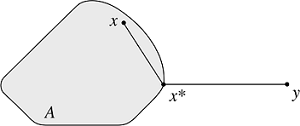
\includegraphics{fig2.png}
\end{center}

This figure shows a point $y$ being projected onto the closed and convex set $A$. By the theorem we just proved and looking at the above diagram, we can observe that the angle resulting from a projection onto a convex set will not necessarily be a right angle. It may be the case, as in the figure, that an obtuse angle (i.e. larger than a 90-degree angle) is obtained. \newline

\subsection{Projection Theorem and Prediction Involving Heterogeneous Variables}

As previously mentioned, the applications of Hilbert spaces (of either finite or infinite dimensions) and their properties are very common in time series analysis and forecasting. Even though the idea of working with data of infinite dimensions may not seem very intuitive or even natural, we can take an extremely large time series dataset and let the number of series tend to infinity. By doing so, we can implicitly work in an infinity dimensional space. \newline

Linear prediction in an infinite dimensional setting has many applications in continuous time processes (i.e. when time $t$ does not only take discrete values). It is also very useful in the study of a large number of time series simultaneously, as it may be the case when analyzing the evolution of a given economy by observing several hundreds of time series that can help explain what is going on in that economy (i.e. GDP, unemployment rate, oil prices, savings rate...). Most of the time, these several hundreds of variables will be heterogeneous, as they may not be identically distributed and might have different nature despite belonging to the same dataset. If the projection theorem still applies under this heterogeneous variable setting, we will be certain that the minimum variance estimator exists. The purpose of this section is to analyze if we can still benefit from the projection theorem and its implications when we have heterogeneous variables by proving the theorem under this scenario. \newline

When we work with linear prediction with heterogeneous variables, we are trying to reduce the sum of squared residuals (i.e. the distance between the observed value and the predicted value for the variable we are estimating). Mathemaically speaking, we are minimizing $\sum_{t=1}^n\lVert Y_t - \theta'X_t \rVert ^2$, where $X_t$ and $Y_t$ are heterogeneous time series variables (hence the subindices $t$) which consist of $n$ observations (i.e. $n$-dimensional vectors). \newline

\begin{thm}[Projection Theorem for heterogeneous variables] \label{thm:htv}
Given the prediction function $\hat{Y_t} = \theta' X_t$, where $Y_t$ and $X_t$ are heterogeneous variables and $\theta \in \Theta \subset A \subset \mathscr{H}$ (i.e. $A$ is a closed and convex subset of a Hilbert space and the parameter space $\Theta$ belongs to $A$), there will exist a unique combination of parameters $\theta'^*$ such that $\theta'^* X_t$ will be the element of smallest norm as it will minimize $\lVert Y_t - \theta' X_t \rVert^2$. $\theta'^*$ will be the least squares estimate for our prediction equation.
\end{thm}

\begin{proof}[Proof of Theorem \ref{thm:htv}]
Let $\delta = \inf {\lVert Y_t - \theta'^* X_t \rVert : \theta'^* X_t \in A}$. If $\theta'^* X_t, Y_t \in A$ then $1/2$$(\theta'^* X_t + Y_t)$ $\in A$ by convexity and, by the parallelogram law, 
\[
\sum_{t=1}^n\lVert Y_t - \theta'^* X_t \rVert^2 = \sum_{t=1}^n [2( \lVert Y_t \rVert^2 + \lVert \theta'^* X_t \rVert^2) - \lVert Y_t +\theta'^* X_t \rVert] \leqslant \sum_{t=1}^n [2(\lVert Y_t \rVert^2 + \lVert \theta'^* X_t \rVert^2) - 4\delta^2].
\]
In the case where $\lVert \theta^* X_t \rVert = \lVert Y_t \rVert = \delta$ then $\sum_{t=1}^n \lVert X_t - Y_t \rVert^2 \leqslant 4\delta^2 - 4\delta^2 = 0$, so $\theta^* X_t = Y_t$ and therefore this point is unique. 
As proved before, an arbitrary sequence in $A$ will be Cauchy and the completeness property is satisfied. Therefore, the least squares estimator $\theta^* X_t$ exists and is unique.
\end{proof}

By the above proof, we can state that the projection theorem applies not only to elements in $\mathbb R^n$ for $n$ finite or infinite but also to vectors of heterogeneous random variables. Consequently, the projection theorem appears to be a very useful result for estimation purposes involving heterogeneous random variables. \newline

\subsection{Application: Convexity of a Time Series Autoregressive (AR) Process}

In statistics and econometrics it is common to model a time series process as an autoregressive process, (i.e. to regress a variable on its previous lags). A variable regressed on its $p$ previous lags will conform an AR($p$) model, an autoregressive model of order $p$. This model can be used to forecast future values of a given variable and takes the form
\[
Y_t = c + \phi_1Y_{t-1} + \phi_2Y_{t-2} + ... + \phi_pY_{t-p} + \epsilon_t,\]
where $c$ is a constant term and $\epsilon_t$ is a white noise shock, a type of covariance stationary \footnote{A \textbf{covariance stationary} process is a time dependent process where all the realized values have the same mean and the covariance between any of these realized values depends on how apart in time they are, and not on the specific time or period they take place.} process that is serially uncorrelated and has constant variance $\sigma_{\epsilon}^2$ and 0 mean. Moreover, AR($p$) processes can be either stationary (i.e. the unconditional joint probability distribution of the process does not change over time) or non-stationary. In this section we will only focus on stationary AR models. Before proving that an AR($p$) process is convex, the following points have to be taken into account:
\begin{enumerate}[(i)]
\item Any AR($p$) process can be put into vector form by rewritting it as $Y_t$ = $A$ $Y_{t-1} + \epsilon_t$, where $A$ is an autoregressive matrix and $Y_{t-1}$ a vector \footnote{The proof of this statement can be found in Time Series Analysis, book by Hamilton (1994).}. In particular, $A$ can also be called \textbf{companion matrix} and it allows us to determine the stationary properties of our process. Equivalently,
  \[
\begin{bmatrix}
    Y_t      \\
    Y_{t-1} \\    
    \vdots \\
    \vdots \\
    Y_{t-p+1}
\end{bmatrix}
= 
\begin{bmatrix}
    \phi_1 & \phi_2 & \cdots & \phi_{p-1} & \phi_p    \\
    1 & 0 & \cdots & 0 & 0 \\     
    0 & 1 & \cdots & 0 & 0 \\
    \vdots & \vdots & \ddots & \vdots & \vdots\\
    0 & 0 & \cdots & 0 & 1
\end{bmatrix} 
\begin{bmatrix}
    Y_{t-1}      \\
    Y_{t-2} \\    
    \vdots \\
    \vdots \\
    Y_{t-p}
\end{bmatrix}
+
\begin{bmatrix}
    \epsilon_t \\
    0 \\
    \vdots \\
    \vdots \\
    0
\end{bmatrix}
\]
We have rewritten an AR($p$) scalar process as a vector autoregression process of order 1, denoted as VAR(1). 

\item A VAR(1) process will be stationary if the largest eigenvalue of the matrix $A$ is smaller than 1 in absolute value \footnote{The proof of this statement can be found in Time Series Analysis, book by Hamilton (1994).}. This will make our AR($p$) model stationary as well. 

\item From basic algebra we know that the following equality holds, \newline
\[ A = T\Lambda T^{-1} \Rightarrow T^{-1}AT = \Lambda = \begin{bmatrix} \lambda_1 & 0 & \cdots & 0\\     
    0 & \lambda_2 & \cdots & 0 \\
    \vdots & \vdots & \ddots & \vdots \\
    0 & 0 & \cdots & \lambda_p \end{bmatrix}, \]
where $\lambda_i$ for $i = 1, ..., p$ correspond to the eigenvalues of the matrix A. 

\item The \textbf{spectral norm} of a matrix $A$, denoted as $\lVert A \rVert$, refers to the largest eigenvalue of $A$ in absolute value.
\end{enumerate}

We need all the eigenvalues of the companion matrix $A$ to be strictly smaller than 1 in absolute value in order to have stationarity. In addition, as we want to ultimately prove that an AR($p$) is convex so that the projection theorem can be applied to this kind of models and the estimator exists and is unique, we also need the matrix $\Lambda$ to have full rank (i.e. rank $p$ as it is a $p \times p$ matrix). Hence, for all $i = 1, ..., p$ we will also need all the eigenvalues to be different from 0. \newline

Now, we define $A_3 = aA_1 + (1 - a)A_2$, where $a \in [0, 1]$ and $A_1$ and $A_2$ are the autoregressive matrices of two stationary VAR(1) processes. To show that an AR($p$) process is convex, we need to prove that the largest eigenvalue of the matrix $A_3$ is smaller than 1 in absolute value. If this condition is satisfied, all the eigenvalues of $A_3$ will be smaller than 1 in absolute value. We have that
\begin{align*}
A_3 &= aA_1 + (1 - a)A_2 = a
\begin{bmatrix}
    \phi_{11} & \phi_{12} & \cdots & \phi_{1p-1} & \phi_{1p}    \\
    1 & 0 & \cdots & 0 & 0 \\     
    0 & 1 & \cdots & 0 & 0 \\
    \vdots & \vdots & \ddots & \vdots & \vdots\\
    0 & 0 & \cdots & 0 & 1
\end{bmatrix} 
+ (1 - a)
\begin{bmatrix}
    \phi_{21} & \phi_{22} & \cdots & \phi_{2p-1} & \phi_{2p}    \\
    1 & 0 & \cdots & 0 & 0 \\     
    0 & 1 & \cdots & 0 & 0 \\
    \vdots & \vdots & \ddots & \vdots & \vdots\\
    0 & 0 & \cdots & 0 & 1
\end{bmatrix} \\
&= 
\begin{bmatrix}
   a \phi_{11} & a \phi_{12} & \cdots & a \phi_{1p-1} & a \phi_{1p}    \\
    a & 0 & \cdots & 0 & 0 \\     
    0 & a & \cdots & 0 & 0 \\
    \vdots & \vdots & \ddots & \vdots & \vdots\\
    0 & 0 & \cdots & 0 & a
\end{bmatrix} 
+
\begin{bmatrix}
    (1 - a) \phi_{21} & (1 - a) \phi_{22} & \cdots & (1 - a) \phi_{2p-1} & (1 - a) \phi_{2p}    \\
    (1 - a) & 0 & \cdots & 0 & 0 \\     
    0 & (1 - a) & \cdots & 0 & 0 \\
    \vdots & \vdots & \ddots & \vdots & \vdots\\
    0 & 0 & \cdots & 0 & (1 - a)
\end{bmatrix}
\end{align*}

To prove convexity, it suffices to work with the expression for the spectral norm of $\lVert A_3 \rVert$, which is a linear combination of the spectral norms of the matrices $A_1$ and $A_2$. By the triangle inequality introduced in the first section and using the fact that $a$ and $(1 - a)$ are non-negative scalars and can be taken outside of the norm, 
\[
\lVert A_3 \rVert = \lVert aA_1 + (1 - a)A_2 \rVert \leqslant \lVert aA_1 \rVert + \lVert (1 - a)A_2 \rVert = a \lVert A_1 \rVert + (1 - a) \lVert A_2 \rVert.
\]
Hence,
\[
\lVert A_3 \rVert \leqslant a \lVert A_1 \rVert + (1 - a) \lVert A_2 \rVert.
\]
We assumed that the two VAR(1) processes associated with the companion matrices $A_1$ and $A_2$ are stationary so all the eigenvalues of these two matrices are, in absolute value, smaller than 1. Consequently, the spectral norms for the matrices $A_1$ and $A_2$ are smaller than 1 in absolute value as well. Further, as $a$ and $(1 - a)$ are at most 1 and the largest eigenvalues of $A_1$ and $A_2$ are smaller or equal than one in absolute value, so is the largest eigenvalue in absolute value of $A_3$. Hence, $\lVert A_3 \rVert < 1$, making the autoregressive process associated with $A_3$ a stationary process. Moreover, since $a \in [0, 1]$, we can conclude that $A_3 = aA_1 + (1 - a)A_2$ is convex. \newline

The convexity of an AR($p$) process and the fact that the coefficients of such specification can be estimated by OLS are very much linked to the projection theorem. As mentioned before, OLS estimation can be interpreted as a projection onto a linear space spanned by the regressors. In particular, due to the fact that an AR($p$) model is convex the projection theorem is helpful when estimating the parameters of the model by OLS and ensures that the resulting estimators exist and are unique. 

\newpage

\section{Conditional Expectation and Best Linear Prediction in $L^2(\Omega, \mathscr{F}, P)$}

After setting the theoretical framework for the projection theorem and even applying some of the results to an autoregressive time series process, now we can relate all those mathematical notions to a more practical issue in statistical forecasting: the best linear prediction. This section shows a very simple application of the projection theorem when predicting a random variable and how it may be able to simplify the process of predicting a given random variable. In the paragraphs below, we work with the probability space and real Hilbert space $L^2(\Omega, \mathscr{F}, P)$ introduced above, the inner-product of which is $\langle X, Y \rangle = \mathbb E(XY)$. Before proceeding, several new concepts must be introduced: \newline


\begin{defn}[Closed span]
The \textbf{closed span} $\bar{sp}\{x_t, t \in T\}$ of any subset ${x_t, t \in T}$ of a Hilbert space $\mathscr{H}$ refers to the smallest closed subspace of such Hilbert space containing each element $x_t, t \in T$. \newline
\end{defn}

\begin{defn}[Best Mean Square Predictor of $Y$]
If $\mathscr{M}$ is a closed subspace of $L^2$ and $Y$ belongs to such subspace, then the \textbf{best mean square predictor} of $Y$ in $\mathscr{M}$ is the element $\hat{Y}$ such that 
\[
\lVert Y - \hat{Y}\rVert^2 = \inf_{X \in \mathscr{M}} \lVert Y - X\rVert^2 = \inf_{X \in \mathscr{M}} \mathbb E| Y - X |^2.
\] 
\end{defn}
By the projection theorem presented in the last section, the unique best predictor of $Y$ in $\mathscr{M}$ is $P_\mathscr{M}$$Y$ = $\hat{Y}$. \newline

\begin{defn}[Conditional Expectation $\mathbb E_{\mathscr{M}}Y$]
If $\mathscr{M}$ is a closed subspace of $L^2$ and if $Y$ $\in$ $L^2$, then the \textbf{conditional expectation of $Y$ given $\mathscr{M}$} is the projection $\mathbb E_{\mathscr{M}}Y=P_\mathscr{M}Y$.
\end{defn}
Further, $\mathbb E_{\mathscr{M}}Y$ is the unique element belonging to $\mathscr{M}$ such that $\mathbb E(W\mathbb E_{\mathscr{M}}Y)=\mathbb E(WY)$. \newline

\begin{defn}[Conditional expectation $\mathbb E(Y|X)$]
Let $X$ be a random variable on $(\Omega, \mathscr{F}, P)$ and Y belong to $L^2(\Omega, \mathscr{F}, P)$, then the \textbf{conditional expectation of $Y$ given $X$} is $\mathbb E(Y|X)$=$\mathbb E_{\mathscr{M}(X)}Y$, where $\mathscr{M}(X)$ is the closed subspace $L^2$ formed by all the random variables contained in $L^2$.
\end{defn}
This definition can be generalized to more than one random variable $X_i$ where $i=1,2...,n$ by conditioning $Y$ on the vector of variables $X_i$. \newline

It must be noted that the inner-product of a $L^2$ space corresponds to a covariance, $\mathbb E(XY)$, and this is what allows us to use the projection theorem to obtain the minimum variance estimator of a vector of finite variance random variables as a function of some other finite variance random variables. Consequently, if both $X$ (or the vector of independent variables) and $Y$ belong to an inner-product space which is well-defined, we do not need to minimize the variance in order to find the best linear predictor. Instead, we can just use the projection theorem to argue that any estimator with orthogonal errors will be the (linear) estimator with minimum variance, as will be developed in a while. More technically: the conditional expectation $\mathbb E_{\mathscr{M}(X_1,...,X_n)}$ is the best mean square predictor of $Y$ in the space $\mathscr{M}(X_1,...,X_n)$, since the squared distance is minimized. \newline

Another way of expressing the notion of best mean square predictor is by saying that $\mathbb E_{\mathscr{M}(X_1,...,X_n)}$ is the best function of $X_1,...,X_n$ in terms of mean square for predicting $Y$. Nevertheless, finding projections on the subspace $\mathscr{M}(X_1,...,X_n)$ is a complex issue. One solution to this problem is to compute the projection of $Y$ on the closed subspan $\bar{sp}\{1, X_1,...,X_n\}$ $\subseteq$ $\mathscr{M}(X_1,...,X_n)$ instead. This will allow us to write
\[
P_{\bar{sp}\{1, X_1,...,X_n\}}(Y) = \sum_{i=0}^{\infty} \alpha_0X_i,
\]
with $X_0=1$ and $\sum_{i=0}^{\infty} \alpha_i\mathbb E(X_iX_j) = \mathbb E(YX_j)$ for $j=1,2,...,n$, where this last expression refers to the \textbf{prediction equation}. \newline

By the projection theorem, we can state that there exists a solution $(\alpha_0,...,\alpha_n)$ which satisfies the above expressions. This is consistent with what has been mentioned before about being able to find the minimum variance estimate of a vector of random variables with finite variance as a function of some other finite variance random variables. By plugging in $P_{\bar{sp}\{1, X_1,...,X_n\}}(Y)$ any solution $(\alpha_0,...,\alpha_n)$ we can obtain the projection we were looking for, which is the \textbf{best linear predictor} of $Y$ in terms of $1,X_1,...,X_n$, denoted by $\hat{Y}$. This projection will have a larger mean squared error than the conditional expectation $\mathbb E_{\mathscr{M}}Y$ but it is more convenient than the conditional expectation as the computations required are less complex. \newline

Given two random variables, $X$ and $Y$, which follow a Gaussian (Normal) distribution and belong to a well-defined inner-product space, the projection of $Y$ onto $X$ corresponds to the conditional expectation $\mathbb E(X|Y)$ and it is linear, making the conditional expectation the best linear prediction. This is equivalent to saying that this remarkable case arises when the vector $(Y,X_1,...,X_n)'$ has a multivariate normal distribution as when this happens, $P_{\bar{sp}\{1, X_1,...,X_n\}}(Y) = \mathbb E_{\mathscr{M}(X_1,...,X_n)}$. However, if at least one of the variables in question is not Gaussian, the projection of $Y$ onto $X$ is the minimum variance linear predicion of $Y$ given $X$ and $\mathbb E(Y|X)$ may not necessarily be linear. \newline

The projection theorem implies that the prediction error will be orthogonal to $X$ (or $X_i$ if we have multiple regressors). Mathematically, for all $X_i \in\mathscr{M}$, 
\[
\langle Y - \hat{Y}, X_i \rangle = 0
\] 

It follows that $\mathbb E(Y - \hat{Y}) = 0$ $\Leftrightarrow$ $\mathbb E [(Y - \hat{Y})X_i] = 0$

Hence, the prediction errors are uncorrelated with the prediction variables $(1, X_1,...,X_n)$. \newline

This final but simple example extracted from \citet{BrockwellDavis:1991} compares the performance of the two predictors, the conditional expectation $E(Y|X)$ and $P_{\bar{sp}\{1,X\}}Y$.

\begin{exmpl}
Suppose $X$ and $Z$ are two independent standard normal random variables and let $Y=X^2 + Z$. The best predictor of $Y$ in terms of $X$ is $\mathbb E(Y|X)=X^2$. Moreover, the best \textit{linear} predictor of $Y$ in terms of $\{1,X\}$ is $P_{\bar{sp}\{1,X\}}Y = aX + b$. Also,
\[
\langle aX+b, X \rangle = \langle Y, X \rangle = \mathbb E(YX) = 0,
\]
\[
\langle aX+b, 1 \rangle = \langle Y, 1 \rangle = \mathbb E(Y) = 1.
\]
From the above equations, we obtain that $a=0$ and $b=1$ and thus $P_{\bar{sp}\{1,X\}}Y = 1$.
\[
\lVert Y - \mathbb E(Y|X)\rVert^2 = \mathbb E(Z^2) = 1.
\]
\[
\lVert Y - P_{\bar{sp}\{1,X\}}Y \rVert^2 = \lVert Y \rVert^2 - 1 = \mathbb E(X^4) + \mathbb E(Z^2) - 1 = 3.
\]
Note that, after comparing the mean squared errors of both predictors, the results are consistent with what has been mentioned above, $\mathbb E(Y|X)$ outperforms $P_{\bar{sp}\{1,X\}}Y$.
\end{exmpl}

\newpage

\section{Conclusions}
After setting the theoretical framework, we were able to present the Hilbert projection theorem (as we evaluated the projection theorem in the context of Hilbert spaces) and its proof. Moreover, such result came with several implications that resulted very useful in other mathematical contexts and even in more practical applications such as statistical forecasting. The main implications of the projection theorem can be summarized in the following points.
\begin{enumerate}[(i)]
\item An element $x$ in a Hilbert space $\mathscr{H}$ can projected onto a closed subspace $\mathscr{M} \in \mathscr{H}$ in a way that the norm or distance between $x$ and the unique projection $\hat{x}$ is minimized. Moreover, the angle between $x$ and $\hat{x}$ will be a 90-degree angle (i.e. we will have an orthogonal projection).
\item We can also project an element $x \in \mathscr{H}$ onto a closed and convex set $A \in \mathscr{H}$ in a way that the norm or distance between such element and its projection $\hat{x}$ is minimized and the projection is unique. Nevertheless, compared to the previous case, orthogonality is not guaranteed anymore because we are now projecting $x$ onto a closed and convex set. Hence, the angle between $x$ and its projection will be either right or obtuse.
\item The projection theorem can also be applied when we are working with heterogeneous variables from a large time series dataset, as we proved. In particular, the projection theorem guarantees the existence and uniqueness of the vector of parameters of a regression, which can be geometrically interpreted as a projection. Those parameters minimize the squared residuals of the regression (i.e. the squared distance between the observed value of the element we are projecting and the predicted value for that element, which corresponds to the projection). 
\end{enumerate}

We also introduced the autoregressive model AR($p$), a common time series specification in statistical forecasting, and proved its convexity. Consequently, we can argue that the projection theorem may be applied when working with such models and that AR($p$) parameters can be estimated by OLS and will be unique. \newline

Finally, we related the concept of best linear prediction to that of projection and introduced the concept of conditional expectation. The best linear predictor and the conditional expectation will not coincide unless $Y$ and the vector of regressors $X$ belong to a well-defined inner-product space and all follow a Gaussian (Normal) distribution.

\newpage

\bibliography{biblio}
\bibliographystyle{natbib}  

\nocite{Hamilton:1994}
\nocite{PeressiniSullivanUhl:1991}
\nocite{Skiadas:2009}
\nocite{DomokosIngramMarsh:2016}
\nocite{Bosq:2014}

\end{document}
